We used a Keypoint-RCNN
\footnote{Pre-trained model available in torchvision: \url{https://pytorch.org/vision/stable/_modules/torchvision/models/detection/keypoint_rcnn.html}}
 to get both bounding boxes of human patches and the keypoints of the humans.
We applied this to every frame in the 2 game training videos and 9 movie training videos, generating 40,000+ samples (Figure \ref{fig:Q1_1}).
We also experimented using a Mask-RCNN
\footnote{Pre-trained model available in torchvision: \url{https://pytorch.org/vision/stable/_modules/torchvision/models/detection/mask_rcnn.html}}
 model to get bounding boxes, but found it tended to give undersized bounding boxes, hence we favour the Keypoint-RCNN.



\begin{figure}[h!]
  \begin{center}
  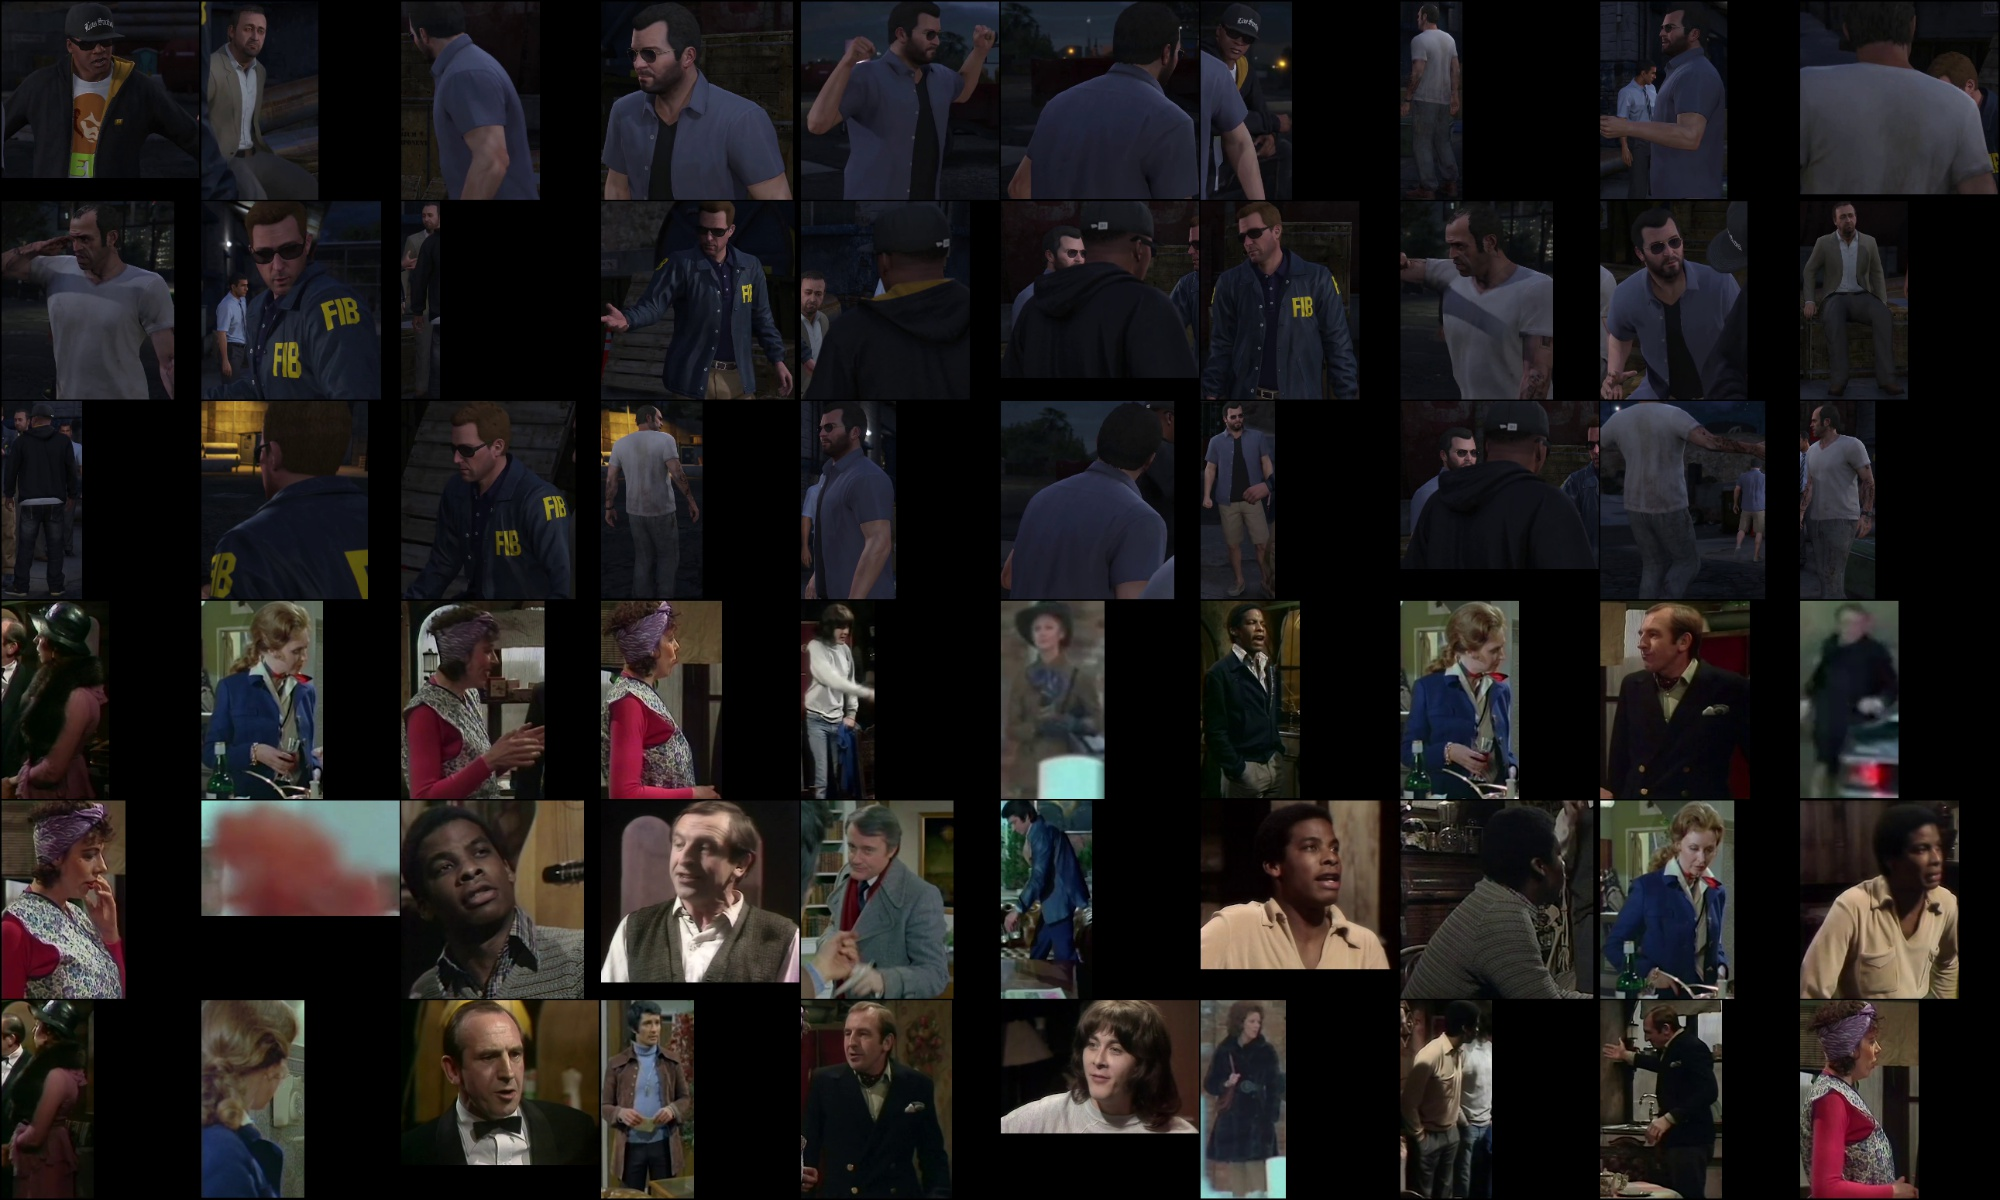
\includegraphics[scale=0.2]{Q1_1_full.jpg}
    \caption{Q1.1 sample of human patches, top game, bottom movie.}
    \label{fig:Q1_1}
  \end{center}
  \end{figure}